% Robert F.K. Martin
% ID 1505151
% CSci 5031
% Homework Set N

\documentclass[11pt]{article}
%\RequirePackage{vmargin}
%\setpapersize{USletter}
%\setmarginsrb{1in}{1.5in}{1in}{0in}{\headheight}{\headsep}{\footheight}{\footskip}
\usepackage{setspace}
\usepackage{homework}
\usepackage{macros}
\usepackage{graphics}
\usepackage{subfigure}
\usepackage{float}
\usepackage{placeins}

% detect interpreter: pdflatex or latex
\newif\ifpdf
\ifx\pdfoutput\undefined
  \pdffalse
\else
  \pdfoutput=1
  \pdftrue
  \pdfcompresslevel=9
\fi

% user: add packages you need
\usepackage{amsmath}

% user: set counter depth for lists
%\setcounter{page}{1}

% user: set style of equation numbering
\numberwithin{equation}{section}  % (sec.number)
\renewcommand{\thetable}{\arabic{table}}
\renewcommand{\thefigure}{\arabic{figure}}

\singlespacing

\begin{document}

% pick type of your preferred page style. UMN requires page numbers.
%\pagestyle{headings}


\noindent Robert F.K. Martin\\
ID 1505151\\
Csci 5523\\
14 Dec 2011\\
Homework 5
\hline
\vspace*{0.25in}
\noindent\textbf{Problem 1a: }

Yes, this scheme will be able to find all the core points(and possibly more). We just need to choose the minimum membership value as our theta. Since fuzzy c-means is a distance based clustering method, the minimum membership values will be near the area between the three clusters.
\vspace*{0.25in}

\noindent\textbf{Problem 1b: }

No, DBSCAN would have a problem finding all the border points. Border points occur wherever a point is near a core point but does not encompass enough other points. This can occur in the middle of a cluster but generally near the edges. Since fuzzy c-clustering is distance-based, it is unlikely that there would be a theta that would define the same clusters and their associated border points the same way as FCM.
\vspace*{0.25in}

\noindent\textbf{Problem 2: }

SNN(A,B)=2; SNN(C,D)=2\\
J(A,B)=$\frac{2}{14}$; J(C,D)=$\frac{2}{6}$ \\
Depending on you definition of intuition, you could have several answers as to which two are the most similar. (A,B) could be more similar because they have more connections in total. In Facebook world, this would be two extroverts from different schools who happen to know each other and they are similar because they are both extroverts. Similarly, we could say (C,D) are more similar because they are both introverts and have few connections. Or, we could say (C,D) are more similar since their few connections in total makes their connection to each other more significant. Depending on the application or metric, any of those answers could be acceptable. But my guess is that this question is set up to show that (C,D) is more similar because of the shared connection among the relatively few total connections.

SNN gives the same similarity for both pairings. The Jaccard ratio gives more importance to (C,D) because of the statistical importance of their shared connection among few connections in total. We could modify the SNN algorithm to report the fraction of shared neighbors among the $k$. This would give (A,B) a score of $\frac{2}{8}$ and (C,D) a score of $\frac{2}{4}$.
\vspace*{0.25in}

\noindent\textbf{Problem 3: }

When there are overlapping clusters of differing densities as found by EM clustering, the silhouette coefficient would not be a good metric. While the within cluster value might be high, the between cluster could be low. As shown in the figure, the differing colors denote different densities.
\FloatBarrier
\begin{figure}[H]
\centering
\subfigure{\resizebox{!}{100mm}{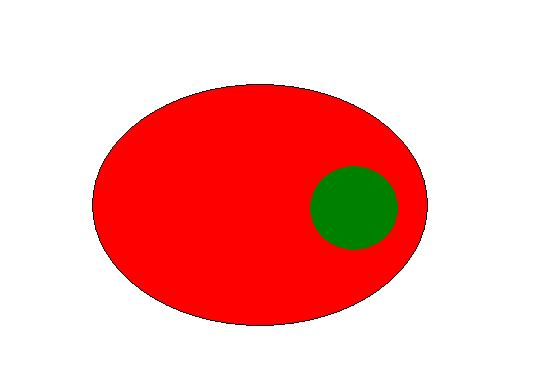
\includegraphics{hw5q3.jpg}}}
\caption{\textbf{Problem 3: }Picture of a problem dataset for silhouette coefficient}
\end{figure}
\FloatBarrier
\vspace*{0.25in}

\noindent\textbf{Problem 4a: }

\FloatBarrier
\begin{figure}[H]
\centering
\subfigure{\resizebox{!}{100mm}{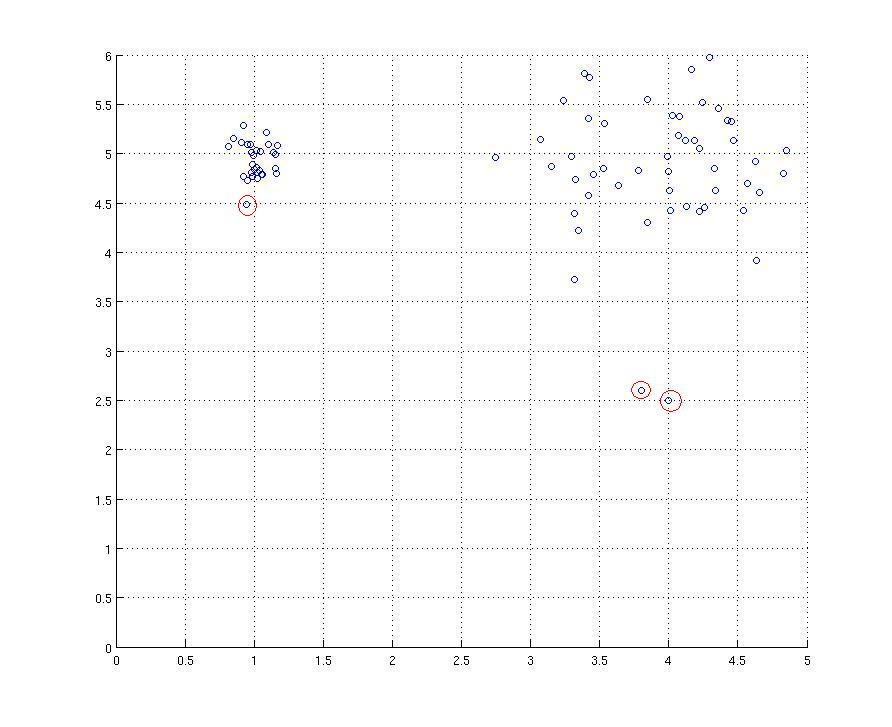
\includegraphics{hw5q4.jpg}}}
\caption{\textbf{Problem 4: }Selected outliers}
\end{figure}
\FloatBarrier

\noindent\textbf{Problem 4b: }

1NN. [4.63 3.92], [3.31 3.73], [4.83 4.80]\\
2NN. [4 2.50], [3.80 2.60], [3.31 3.73]\\
10NN. [4 2.50], [3.80 2.60], [3.31 3.73].
\vspace*{0.25in}

\noindent\textbf{Problem 4c: }

[0.940 4.48], [4 2.50], [3.80 2.60]
\vspace*{0.25in}

\noindent\textbf{Problem 4d: }

kNN has trouble finding outliers if there are clusters of differing densities.
\vspace*{0.25in}

\noindent\textbf{Problem 5: }

A similarity between both proximity- and clustering-based anomaly detection is that they are both simple and use well-known techniques we have already studied.\\

A difference is that proximity anomaly detection relies on some concept of distance where clustering-based detection is more flexible and can use density or graph based approaches to building clusters.
\vspace*{0.25in}

\noindent\textbf{Problem 6: }

One advantage is that this new algorithm is a single-pass technique. We only need to pass through one clustering step. Whereas the K-means algorithm not only needs to do the clustering but also measure the median distance of all points in a cluster and find the relative distance of all points in a cluster.\\

A disadvatange of this scheme is that possibly just less than half the points may end up being outliers.\\

We could add an additional computation by taking the distance of a point to the non-outlier cluster divided by the distance to the outlier cluster. High scores will be outliers and low scores will be part of the non-outlier cluster.
\vspace*{0.25in}

\end{document}










